%
% This is the LaTeX template file for lecture notes for EE 382C/EE 361C.
%
% To familiarize yourself with this template, the body contains
% some examples of its use.  Look them over.  Then you can
% run LaTeX on this file.  After you have LaTeXed this file then
% you can look over the result either by printing it out with
% dvips or using xdvi.
%
% This template is based on the template for Prof. Sinclair's CS 270.

\documentclass[twoside]{article}
\usepackage{graphicx}
\usepackage{listings}
\setlength{\oddsidemargin}{0.25 in}
\setlength{\evensidemargin}{-0.25 in}
\setlength{\topmargin}{-0.6 in}
\setlength{\textwidth}{6.5 in}
\setlength{\textheight}{8.5 in}
\setlength{\headsep}{0.75 in}
\setlength{\parindent}{0 in}
\setlength{\parskip}{0.1 in}

%
% The following commands set up the lecnum (lecture number)
% counter and make various numbering schemes work relative
% to the lecture number.
%
\newcounter{lecnum}
\renewcommand{\thepage}{\thelecnum-\arabic{page}}
\renewcommand{\thesection}{\thelecnum.\arabic{section}}
\renewcommand{\theequation}{\thelecnum.\arabic{equation}}
\renewcommand{\thefigure}{\thelecnum.\arabic{figure}}
\renewcommand{\thetable}{\thelecnum.\arabic{table}}

%
% The following macro is used to generate the header.
%
\newcommand{\lecture}[4]{
   \pagestyle{myheadings}
   \thispagestyle{plain}
   \newpage
   \setcounter{lecnum}{#1}
   \setcounter{page}{1}
   \noindent
   \begin{center}
   \framebox{
      \vbox{\vspace{2mm}
    \hbox to 6.28in { {\bf EE 382C/361C: Multicore Computing
                        \hfill Fall 2016} }
       \vspace{4mm}
       \hbox to 6.28in { {\Large \hfill Lecture #1: #2  \hfill} }
       \vspace{2mm}
       \hbox to 6.28in { {\it Lecturer: #3 \hfill Scribe: #4} }
      \vspace{2mm}}
   }
   \end{center}
   \markboth{Lecture #1: #2}{Lecture #1: #2}
   %{\bf Disclaimer}: {\it These notes have not been subjected to the
   %usual scrutiny reserved for formal publications.  They may be distributed
   %outside this class only with the permission of the Instructor.}
   \vspace*{4mm}
}

%
% Convention for citations is authors' initials followed by the year.
% For example, to cite a paper by Leighton and Maggs you would type
% \cite{LM89}, and to cite a paper by Strassen you would type \cite{S69}.
% (To avoid bibliography problems, for now we redefine the \cite command.)
% Also commands that create a suitable format for the reference list.
\renewcommand{\cite}[1]{[#1]}
\def\beginrefs{\begin{list}%
        {[\arabic{equation}]}{\usecounter{equation}
         \setlength{\leftmargin}{2.0truecm}\setlength{\labelsep}{0.4truecm}%
         \setlength{\labelwidth}{1.6truecm}}}
\def\endrefs{\end{list}}
\def\bibentry#1{\item[\hbox{[#1]}]}

%Use this command for a figure; it puts a figure in wherever you want it.
%usage: \fig{NUMBER}{SPACE-IN-INCHES}{CAPTION}
\newcommand{\fig}[3]{
			\vspace{#2}
			\begin{center}
			Figure \thelecnum.#1:~#3
			\end{center}
	}
% Use these for theorems, lemmas, proofs, etc.
\newtheorem{theorem}{Theorem}[lecnum]
\newtheorem{lemma}[theorem]{Lemma}
\newtheorem{proposition}[theorem]{Proposition}
\newtheorem{claim}[theorem]{Claim}
\newtheorem{corollary}[theorem]{Corollary}
\newtheorem{definition}[theorem]{Definition}
\newenvironment{proof}{{\bf Proof:}}{\hfill\rule{2mm}{2mm}}

% **** IF YOU WANT TO DEFINE ADDITIONAL MACROS FOR YOURSELF, PUT THEM HERE:
\lstdefinestyle{mystyle}{
  captionpos=b
}
\lstset{style=mystyle}
\renewcommand\lstlistingname{Code}

\graphicspath{{images/}}

\begin{document}
%FILL IN THE RIGHT INFO.
%\lecture{**LECTURE-NUMBER**}{**DATE**}{**LECTURER**}{**SCRIBE**}
\lecture{15}{October 18}{Vijay Garg}{Ben Fu}
%\footnotetext{These notes are partially based on those of Nigel Mansell.}

% **** YOUR NOTES GO HERE:

% Some general latex examples and examples making use of the
% macros follow.  
%**** IN GENERAL, BE BRIEF. LONG SCRIBE NOTES, NO MATTER HOW WELL WRITTEN,
%**** ARE NEVER READ BY ANYBODY.
\section{Introduction}
The lecture introduces the concept of {\em scan}, or {\em prefix-sum}. Scan is first defined and later implemented using three different algorithms.

\section{Scanning Algorithms}

A {\em scan} algorithm, also known as a {\em prefix-sum} algorithm, takes a binary associative operator $\oplus$ and an array of $n$ elements:
\begin{center}
$$[a_0, a_1, a_2, ..., a_{n-1}]$$\newline
\end{center}

and returns the array with the operator applied cumulatively such as follows:
\begin{center}
$$[a_0, a_0 \oplus a_1, a_0 \oplus a_1 \oplus a_2, ..., a_0 \oplus a_1 \oplus a_2 \oplus ... \oplus a_{n-1}]$$\newline
\end{center}

For example, if the operator $\oplus$ is addition and we have an array such as follows:
\begin{center}
$$[3, 1, 7, 0, 4, 1, 6, 3]$$\newline
\end{center}

the result of the scan, or prefix-sum, would be the array:
\begin{center}
$$[3, 4, 11, 11, 15, 16, 22, 25]$$\newline
\end{center}

For simplicity, we will use addition as the operator $\oplus$ when discussing the following algorithms.



\subsection{Sequential Scan}
Naturally, the sequential algorithm is to iterate through the array, applying the operator to each new element. The pseudocode for the sequential algorithm is as follows [1]:

\begin{lstlisting}[caption=Sequential Scan]
out[0] = in[0]
for all i from 1 to n
    out[i] = out[i-1] + in[i]
\end{lstlisting}

The time and work complexity for this algorithm are both O(n).



\subsection{Hillis-Steele Scan}

The second algorithm was introduced by Hillis and Steele, which is a naive parallel implementation of the sequential scan algorithm. The naive parallel algorithm is as follows[1]:

\begin{lstlisting}[caption=Hillis-Steele Scan, mathescape]
out[0] = in[0]
for all i from 1 to log(n)
    for all k in parallel
        if k $\geq$ $2^d$ then $x[k - 2^{d-1}] + x[k]$
\end{lstlisting}

\begin{figure}[h]
    \centering
    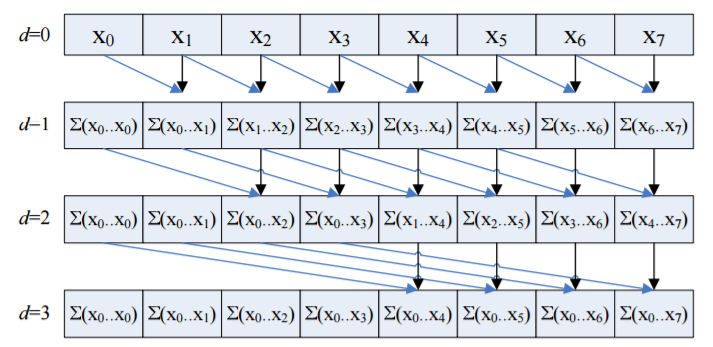
\includegraphics{naive}
    \caption{Hillis-Steele naive parallel scan}
    \label{fig:hillis-steele}
\end{figure}
\break

The algorithm is correct but not work optimal. The total number of operations the algorithm performs is $O(nlogn)$, which is sub-optimal.


\subsection{Blelloch Scan}

To build a work-optimal solution to scan, we use a balanced binary tree. Although an actual data structure is not allocated, the solution builds partial sums that can be represented by a balanced binary tree. In this solution, which was formed by Blelloch [2], there are two phases: an {\em upsweep} and a {\em downsweep} phase.

In the upsweep phase, each thread computes the partial sums of the two lower-level elements. This can be visualized by the following figure:

\begin{figure}[h]
    \centering
    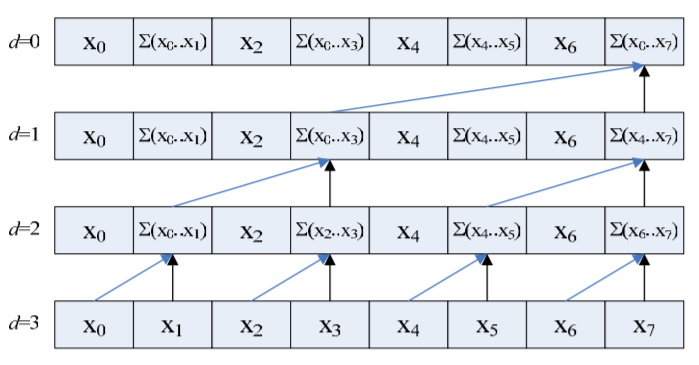
\includegraphics{upsweep}
    \caption{Upsweep phase in Blelloch Scan}
    \label{fig:upsweep}
\end{figure}
\break

The algorithm is as follows [1]:

\begin{lstlisting}[caption=Upsweep Phase, mathescape]
for all d from 0 to log(n-1)
    for all k from 0 to n-1 by $2^{d+1}$ in parallel
        $x[k + 2^{d+1} - 1] = x[k + 2^d - 1] + x[k + 2^{d + 1} - 1]$
\end{lstlisting}

In the downsweep phase, we build the scan using the partial sums computed during the upsweep phase, replacing the elements with the scan output in place. Note that the example provided is an exclusive scan; that is, a zero is inserted into the first step of the downsweep and the final array does not include the total sum.

\begin{figure}[h]
    \centering
    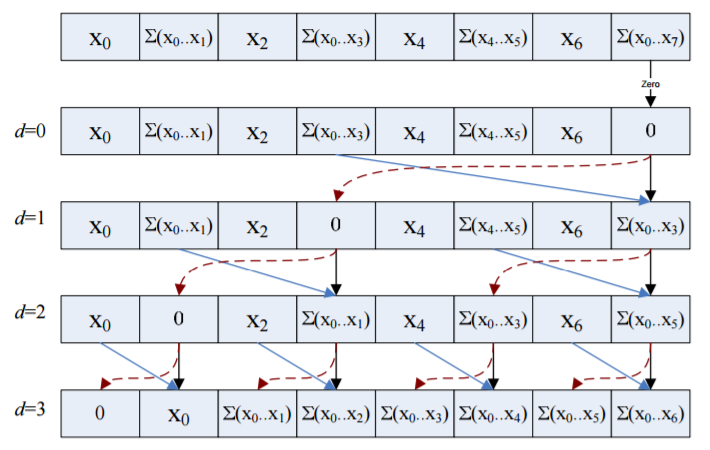
\includegraphics{downsweep}
    \caption{Downsweep phase in Blelloch Scan}
    \label{fig:downsweep}
\end{figure}
\break

The algorithm is as follows:

\begin{lstlisting}[caption=Downsweep Phase, mathescape]
x[n - 1] = 0
for all d from log(n) down to 0
    for all k from 0 to n-1 by $2^{d+1}$ in parallel
        $temp = x[k + 2^d - 1]$
        $x[k + 2^d - 1] = x[k + 2^{d + 1} - 1]$
        $x[k + 2^{d+1} - 1] = temp + x[k + 2^{d + 1} - 1]$
\end{lstlisting}

A sample implementation of the Blelloch algorithm in CUDA C code is shown on the next page.
\newpage
\begin{figure}[h!]
    \centering
    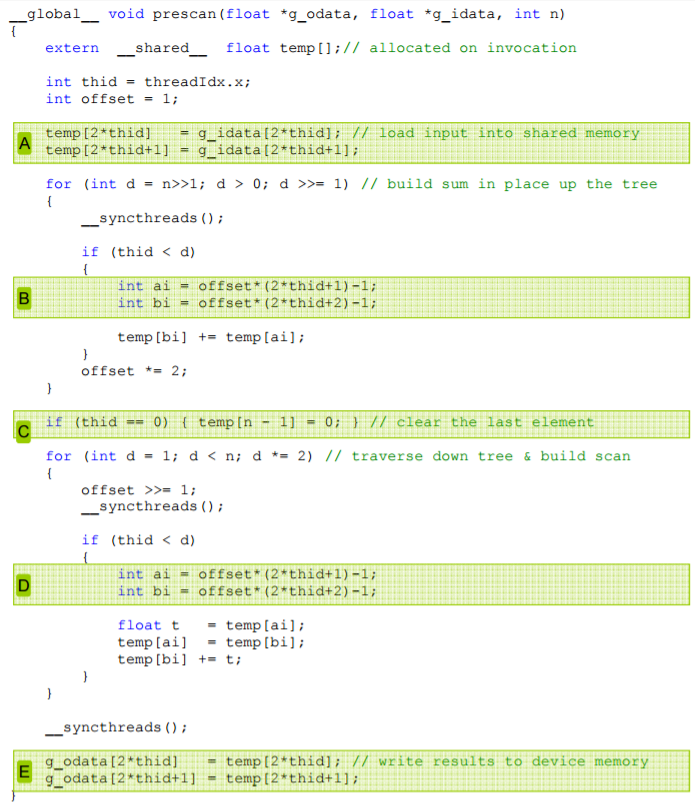
\includegraphics{cuda-blelloch}
    \caption{CUDA implementation for Blelloch Scan}
    \label{fig:cuda-blelloch}
\end{figure}
\newpage


\subsection{Complexity Table}
The complexity table for the time and work complexities of the previous three algorithms are shown in the following table:

\begin{table}[h]
\centering
\begin{tabular}{||c c c||} 
 \hline
 Scan Algorithm & Time Complexity & Work Complexity \\ [0.5ex] 
 \hline\hline
 Sequential & $O(n)$ & $O(n)$  \\ 
 \hline
 Hillis-Steele & $O(log(n))$ & $O(nlog(n))$ \\
 \hline
 Blelloch (Work Optimal) & $O(log(n))$ & $O(n)$ \\
 \hline
\end{tabular}
    \caption{Analysis of Scan Algorithms}
    \label{tab:analysis}
\end{table}


\section*{References}
\beginrefs
\bibentry{1}{\sc M. Harris}, Parallel Prefix Sum (Scan) with CUDA,
{\it Nvidia Corporation\/} (2007),
pp.~3--10.

\bibentry{2}{\sc G. E. Blelloch}, Prefix Sums and Their Applications,
{\it Synthesis of Parallel Algorithms\/} (1990).
\endrefs


\end{document}





